% Paquets généraux
\documentclass[a4paper,12pt,titlepage]{article}
\usepackage[T1]{fontenc}
\usepackage[utf8]{inputenc}
\usepackage[french]{babel}
\usepackage[gen]{eurosym}
%\usepackage[dvips]{graphicx}
\usepackage{fancyhdr}
\usepackage{pdfpages} 
\usepackage{multido}
\usepackage{hyperref}
%\usepackage{textcomp}
%\usepackage{aeguill}
\usepackage{schemabloc}
\usepackage[bitstream-charter]{mathdesign}

\newcommand{\id}{54}
\newcommand{\nom}{Liaisons mécaniques}
\newcommand{\sequence}{04}
\newcommand{\num}{01}
\newcommand{\type}{TP}
\newcommand{\descrip}{Modélisation d'un solide. Comportement des liaisons mécaniques. Modéliser les mécanismes du laboratoire par un schéma cinématique, paramétré.}
\newcommand{\competences}{A3-C4: Analyse d'architecture et de comportement \\ &  Mod1-C1: Isolement d'un solide ou d'un système de solides \\ &  Mod2-C10-1: Modèle de solide indéformable \\ &  Mod2-C11: Modélisation géométrique et cinématique des mouvements entre solides indéformables \\ &  Mod2-C12: Modélisation cinématique des liaisons entre solides \\ &  Mod2-C15: Modélisation des actions mécaniques \\ &  Rés-C6: Utilisation d'un solveur ou d'un logiciel multi physique \\ &  Com1-C1: Différents descripteurs introduits dans le programme \\ &  Com2-C4: Outils de communication}
\newcommand{\nbcomp}{9}
\newcommand{\systemes}{Plateforme Stewart}
\newcommand{\systemessansaccent}{Plateforme Stewart}
\newcommand{\ilot}{2}
\newcommand{\ilotstr}{02}
\newcommand{\dossierilot}{\detokenize{Ilot_02 Plateforme Stewart}}
\newcommand{\imageun}{Plateforme}

\newcommand{\urlsysteme}{\href{https://www.costadoat.fr/systeme/57}{Ressources système}}
\newcommand{\matlabsimscape}{\href{https://github.com/Costadoat/Sciences-Ingenieur/raw/master/Systemes/Plateforme Stewart/Plateforme_Stewart_Simscape.zip}{Modèle Simscape}}
\newcommand{\solidworks}{\href{https://github.com/Costadoat/Sciences-Ingenieur/raw/master/Systemes/Plateforme Stewart/Plateforme_Stewart_Solidworks.zip}{Modèle Solidworks}}
\newcommand{\edrawings}{\href{https://github.com/Costadoat/Sciences-Ingenieur/raw/master/Systemes/Plateforme Stewart/Plateforme_Stewart.EASM}{Modèle eDrawings}}
\newcommand{\test}{Stewart_param1}
\newcommand{\testi}{Stewart_param2}
\newcommand{\testii}{Stewart_param3}
\newcommand{\testiii}{Stewart_param4}
\newcommand{\testiiii}{Stewart_euler}

\newcommand{\auteurun}{Renaud Costadoat}
\newcommand{\auteurdeux}{Françoise Puig}
\newcommand{\institute}{Lycée Dorian}


\usepackage{color}
\usepackage{xcolor}
\usepackage{colortbl}
\usepackage{helvet}
\renewcommand{\familydefault}{\sfdefault}
\usepackage{amsfonts}
\usepackage{amsmath}
%\usepackage{xspace}
\usepackage{varioref}
\usepackage{tabularx}
%\usepackage{floatflt}
\usepackage{graphics}
\usepackage{wrapfig}
\usepackage{textcomp}
\usepackage{tikz}
\usepackage{wrapfig}
\usepackage{gensymb}
\usepackage[european]{circuitikz}
\usetikzlibrary{babel}
\usepackage{ifthen}
\usepackage{cancel}
\usepackage{etoolbox}
\usepackage{multirow}
%\usepackage{boxedminipage}
\definecolor{gris25}{gray}{0.75}
\definecolor{bleu}{RGB}{18,33,98}
\definecolor{bleuf}{RGB}{42,94,171}
\definecolor{bleuc}{RGB}{231,239,247}
\definecolor{rougef}{RGB}{185,18,27}
\definecolor{rougec}{RGB}{255,188,204}%255,230,231
\definecolor{vertf}{RGB}{103,126,82}
\definecolor{vertc}{RGB}{220,255,191}
\definecolor{forestgreen}{rgb}{0.13,0.54,0.13}
\definecolor{blcr}{rgb}{0.59,0.69,0.84}
\definecolor{blfr}{rgb}{0.32,0.51,0.75}
\definecolor{orfr}{rgb}{0.90,0.42,0.15}
\definecolor{orcr}{rgb}{0.90,0.65,0.50}
\definecolor{orangef}{rgb}{0.659,0.269,0.072}
\definecolor{orange}{rgb}{0.58,0.35,0.063}
\definecolor{orangec}{rgb}{0.43,0.32,0.25}
\definecolor{rcorrect}{rgb}{0.6,0,0}
\definecolor{sequence}{rgb}{0.75,0.75,0.75}
\definecolor{competences}{rgb}{0.61,0.73,0.35}
\definecolor{grisf}{HTML}{222222}
\definecolor{grisc}{HTML}{636363}
\definecolor{normal}{HTML}{4087c4}
\definecolor{info}{HTML}{5bc0de}
\definecolor{success}{RGB}{92,184,92}
\definecolor{warning}{RGB}{240,173,78}
\definecolor{danger}{RGB}{217,83,79}
\hypersetup{                    % parametrage des hyperliens
    colorlinks=true,                % colorise les liens
    breaklinks=true,                % permet les retours à la ligne pour les liens trop longs
    urlcolor= blfr,                 % couleur des hyperliens
    linkcolor= orange,                % couleur des liens internes aux documents (index, figures, tableaux, equations,...)
    citecolor= forestgreen                % couleur des liens vers les references bibliographiques
    }

% Mise en page
\pagestyle{fancy}

\setlength{\hoffset}{-18pt}

\setlength{\oddsidemargin}{0pt} 	% Marge gauche sur pages impaires
\setlength{\evensidemargin}{0pt} 	% Marge gauche sur pages paires
\setlength{\marginparwidth}{00pt} 	% Largeur de note dans la marge
\setlength{\headwidth}{481pt} 	 	% Largeur de la zone de tête (17cm)
\setlength{\textwidth}{481pt} 	 	% Largeur de la zone de texte (17cm)
\setlength{\voffset}{-18pt} 		% Bon pour DOS
\setlength{\marginparsep}{7pt}	 	% Séparation de la marge
\setlength{\topmargin}{-30pt} 		% Pas de marge en haut
\setlength{\headheight}{35pt} 		% Haut de page
\setlength{\headsep}{20pt} 		% Entre le haut de page et le texte
\setlength{\footskip}{30pt} 		% Bas de page + séparation
\setlength{\textheight}{700pt} 		% Hauteur de l'icone zone de texte (25cm)
\setlength\fboxrule{1 pt}
\renewcommand{\baselinestretch}{1}
\setcounter{tocdepth}{1}
\newcommand{\cadre}[2]
{\fbox{
  \begin{minipage}{#1\linewidth}
   \begin{center}
    #2\\
   \end{center}
  \end{minipage}
 }
}

\newcounter{num_quest} \setcounter{num_quest}{0}
\newcounter{num_rep} \setcounter{num_rep}{0}
\newcounter{num_cor} \setcounter{num_cor}{0}

\newcommand{\question}[1]{\refstepcounter{num_quest}\par
~\ \\ \parbox[t][][t]{0.15\linewidth}{\textbf{Question \arabic{num_quest}}}\parbox[t][][t]{0.93\linewidth}{#1}\par
}


\newcommand{\reponse}[1]
{\refstepcounter{num_rep}
\noindent
\rule{\linewidth}{.5pt}
\textbf{Question \arabic{num_rep}:}
\multido{\i=1+1}{#1}{~\ \\}
}

\newcommand{\cor}
{\refstepcounter{num_cor}
\noindent
\rule{\linewidth}{.5pt}
\textbf{Question \arabic{num_cor}:} \\
}

\newcommand{\titre}[1]
{\begin{center}
\cadre{0.8}{\huge #1} 
\end{center}
}


% En tête et pied de page
\fancypagestyle{normal}{%
  \fancyhf{}
\lhead{\nom}
\rhead{
\includegraphics[width=2cm]{../../img/logo}\hspace{2pt}}
\ifdef{\auteurdeux}{\lfoot{\auteurun,\auteurdeux}}{\lfoot{\auteurun}}
\cfoot{Page \thepage}}

\fancypagestyle{correction}{%
  \fancyhf{}
  \lhead{\colorbox{danger}{\begin{minipage}{0.65\paperwidth} \textcolor{white}{\textbf{Correction}} \end{minipage}} }
  \rhead{
\includegraphics[width=2cm]{../../img/logo}}
  \ifdef{\auteurdeux}{\lfoot{\auteurun,\auteurdeux}}{\lfoot{\auteurun}}
  \rfoot{\colorbox{danger}{\begin{minipage}{0.5\paperwidth} \begin{flushright}\textcolor{white}{\textbf{Correction}}\end{flushright} \end{minipage}} }}

\renewcommand{\footrulewidth}{0.4pt}

\usepackage{eso-pic}
\newcommand{\BackgroundPic}{%
\put(0,0){%
\parbox[b][\paperheight]{\paperwidth}{%
\vfill
\begin{center}
\hspace{0.5cm}\vspace{0.5cm}

\includegraphics[width=\paperwidth,height=\paperheight,%
keepaspectratio]{../../img/fond3}%
\end{center}
\vfill
}}}

\newcommand{\BackgroundPicdeux}{%
\put(25,-30){%
\parbox[b][\paperheight]{\paperwidth}{%
\vfill
\begin{center}
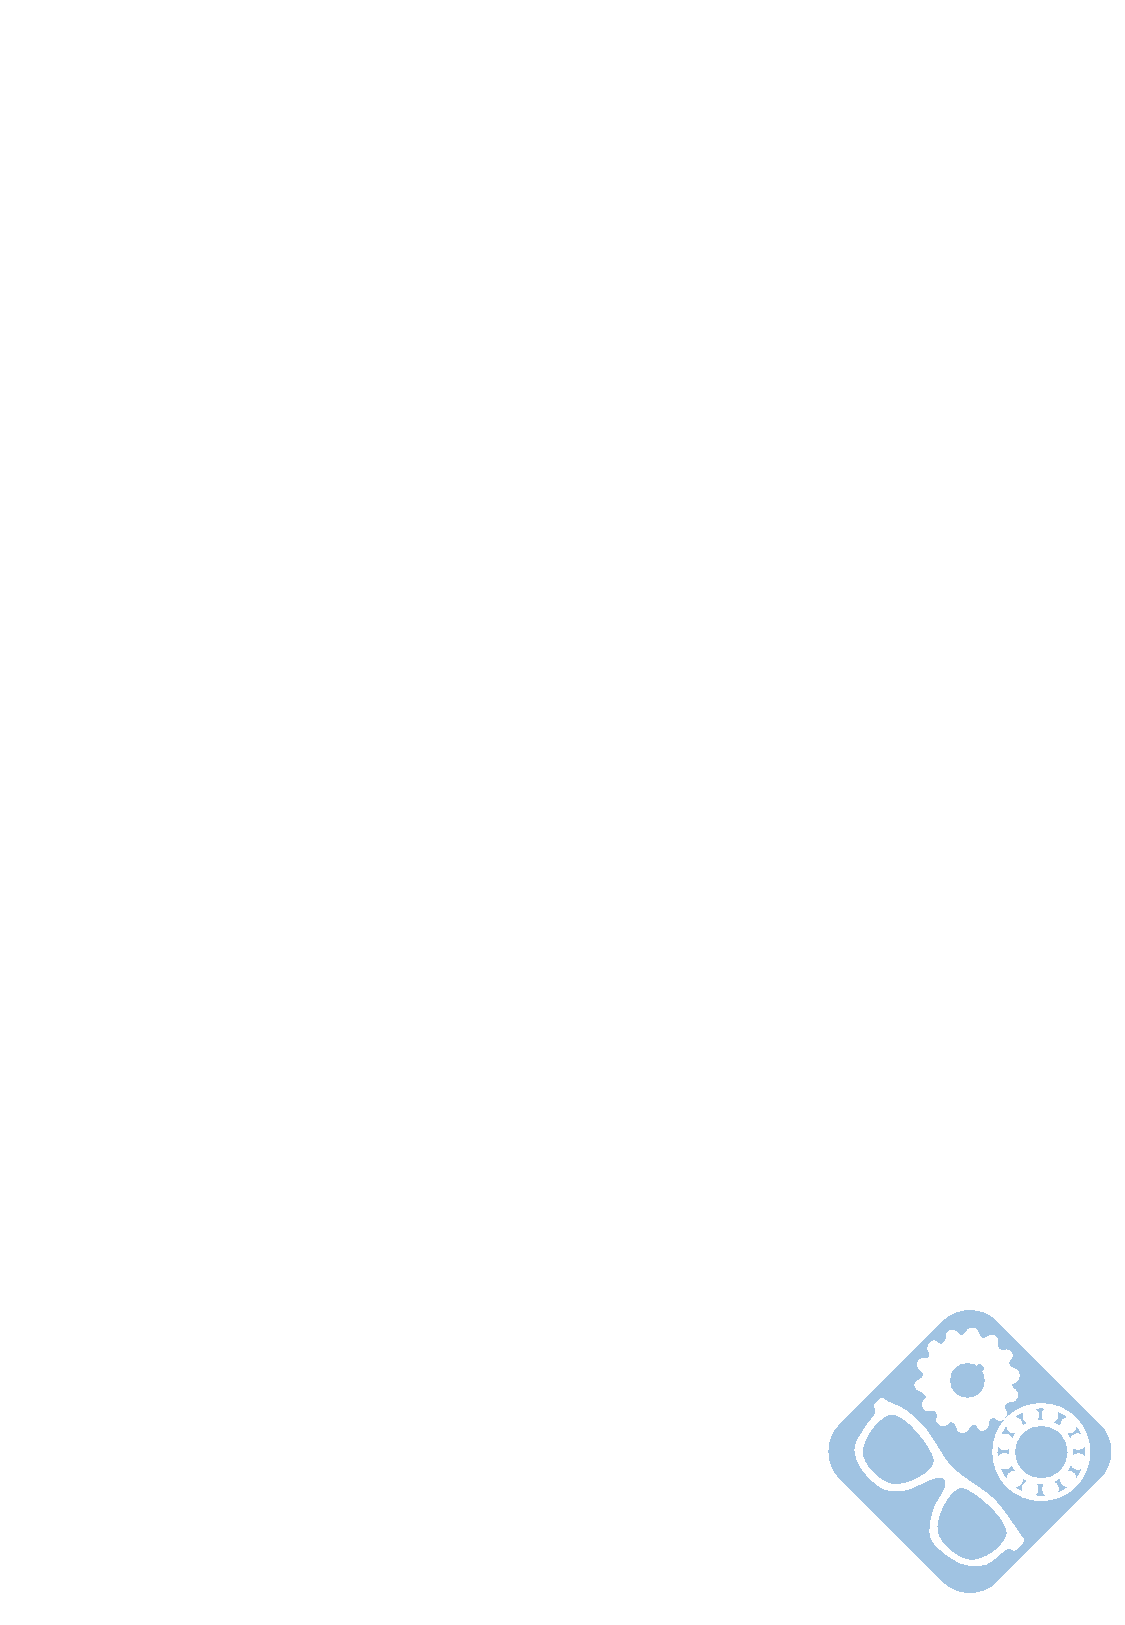
\includegraphics[width=\paperwidth,height=\paperheight,%
keepaspectratio]{../../img/fond4}%
\end{center}
\vfill
}}}

\begin{document}

\pagestyle{empty}

\vspace*{-3\baselineskip}

\AddToShipoutPicture*{\BackgroundPic}

\ifdef{\auteurdeux}{\begin{tabular}{>{\columncolor{gray!00}}m{.3\linewidth} m{.3\linewidth} >{\columncolor{gray!00}}m{.3\linewidth}}
Séquence : \sequence &  \multirow{3}{*}{\hspace{1cm}
\includegraphics[height=1.5cm]{../../img/logo}} &  \begin{flushright} \multirow{4}{*}{\hspace{1cm}
\includegraphics[height=4cm]{img/qrcode}}\end{flushright}\\
Document : \type\num \\
 \institute \\
 \auteurun\\
 \auteurdeux
\end{tabular}}{\begin{tabular}{>{\columncolor{gray!00}}m{.3\linewidth} m{.3\linewidth} >{\columncolor{gray!00}}m{.3\linewidth}}
Séquence : \sequence &  \multirow{3}{*}{\hspace{1cm}
\includegraphics[height=1.5cm]{../../img/logo}} &  \begin{flushright} \multirow{4}{*}{\hspace{1cm}
\includegraphics[height=4cm]{img/qrcode}}\end{flushright}\\
Document : \type\num \\
 \institute \\
 \auteurun
\end{tabular}}

\vspace{1cm}

\ifdef{\prive}{\begin{center}\colorbox{danger}{\Huge{Avec Correction}}\end{center}}{}

\begin{center}\huge{\nom}\end{center}

\vspace{2cm}

\ifdef{\imagedeux}{\begin{minipage}{0.49\linewidth}}{}
\begin{center}\includegraphics[height=5cm]{/home/renaud/Documents/Renaud/GitHub/django_education/systemes/\imageun}\end{center}
\ifdef{\imagedeux}{\end{minipage}\hfill
\begin{minipage}{0.49\linewidth}
\begin{center}\includegraphics[height=5cm]{/home/renaud/Documents/Renaud/GitHub/django_education/systemes/\imagedeux}\end{center}
\end{minipage}}{}

\vspace{5cm}


\begin{tabular}{p{.15\linewidth} >{\columncolor{white}}p{.8\linewidth}}
    \rowcolor{gray!20}
    Référence & S\sequence\ - \type\num \\
    Compétences & \competences \\
 	\rowcolor{gray!20}
    Description & \descrip \\
    Système & \systemes
  \end{tabular}

\newpage

\AddToShipoutPicture{\BackgroundPicdeux}

\pagestyle{normal}

\section{Colleuse de lamelle}

\subsection{Présentation}

\begin{figure}[!h]
  \begin{minipage}{0.35\linewidth}
  \centering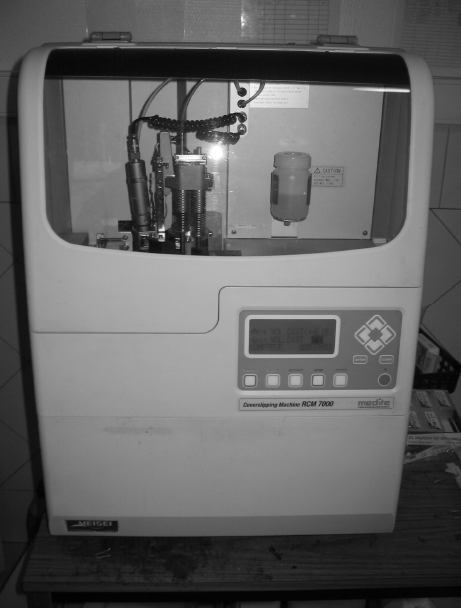
\includegraphics[width=0.8\linewidth]{img/colleuse.png}
  \caption{Colleuse}
  \label{img1}
  \end{minipage}
  \hfill
  \begin{minipage}{0.60\linewidth}
  Le groupe TECH-INTER commercialise du matériel de laboratoire d'histopathologie. Cette spécialité médicale consiste à découper des tissus d'organes en fine épaisseur ($4-5 \mu m$). Ces tissus sont ensuite collés sur des lames de verres de 2 mm d'épaisseur puis colorés chimiquement dans un automate. Pour certains tissus, il est nécessaire de coller sur les tissus colorés une lamelle de verre de 0,3 mm d'épaisseur afin de les protéger (photo 3 document 2). Cette dernière opération est très délicate à effectuer manuellement et très longue, une étude pouvant comporter plusieurs centaines de lames.

  L'appareil appelé « Colleuse de lamelle » automatise ce procédé, figure \ref{img1}.
\end{minipage}
\end{figure}

\subsection{Analyse statique de l'élévateur de rack}

Le schéma cinématique, figure 6 document 6) représente le système d'élévateur de rack. Un moteur non représenté exerce sur l'axe 10 un couple moteur Cm inconnu, ce dernier entraîne par un système vis-écrou comportant un pas à droite, le support de rack 11 qui supporte une charge P connue. Les poids sont négligés. Le système est considéré comme spatial.

Le mouvement étant très lent, on peut supposer que l'ensemble est à l'équilibre par rapport au repère galiléen R0 . Le but est de valider le couple moteur choisi par le constructeur.

Le couple moteur nominal en charge est égal à 1 N.m. pour une charge P = 100N.

Les liaisons sont supposées parfaites.

Les torseurs couple moteur et charge sont les suivants :

\begin{figure}[!h]
  \begin{minipage}{0.35\linewidth}
  \begin{math}
  \left\{F_{mot \rightarrow 10}\right\}=\left\{
  \begin{array}{c c}
  0 & 0 \\
  0 & C_m \\
  0 & 0
  \end{array}\right\}_{(O,R_0)}
  \end{math}
  \end{minipage}
  \hfill
  \begin{minipage}{0.60\linewidth}
  \begin{math}
  \left\{F_{charge \rightarrow 11}\right\}=\left\{
  \begin{array}{c c}
  0 & 0 \\
  -P & 0 \\
  0 & 0
  \end{array}\right\}_{(O,R_0)}
  \end{math}
\end{minipage}
\end{figure}

\paragraph{Question 1:} A partir du schéma cinématique de la figure \ref{img2}, établir le graphe de liaison du mécanisme.

\paragraph{Question 2:} Identifier et écrire le torseur statique de chaque liaison.

Donner une équation supplémentaire en fonction des caractéristiques du torseur pour la liaison hélicoïdale, faisant intervenir le pas p du filetage.

\paragraph{Question 3:} Écrire les torseurs statiques $\left\{T'_{0 \rightarrow 11}\right\}_B$ et $\left\{T''_{0 \rightarrow 11}\right\}_C$ au point O, indiquer les calculs des moments.

\paragraph{Question 4:} Isoler le solide 10. Faire le Bilan des Actions Mécaniques et déterminer les 6 équations d'équilibre du solide 10 (moments au point O).

\paragraph{Question 5:} Isoler le solide 11. Faire le Bilan des Actions Mécaniques et déterminer les 6 équations d'équilibre du solide 11 (moments au point O).

\paragraph{Question 6:} Déterminer le couple moteur Cm en fonction de la charge P et du pas p.

A.N. : calculer $C_m$ pour $p = 6,28 mm$ (pour un tour) et $P = 100 N$. Conclure.

\begin{figure}[!h]
  \centering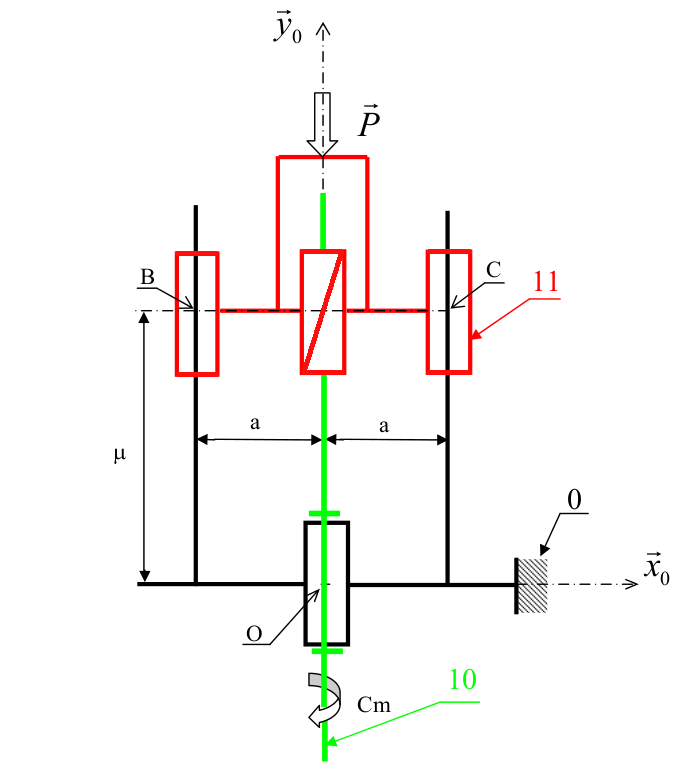
\includegraphics[width=0.6\linewidth]{img/colleuse_cin.png}
  \caption{Schéma cinématique}
  \label{img2}
\end{figure}

\newpage

\section{Démarreur D6RA}

\subsection{Présentation}
Un moteur thermique doit être entraîné en rotation afin de lui faire atteindre son cycle de fonctionnement, c'est le rôle du démarreur.

Pour atteindre son cycle d'auto-fonctionnement, un moteur thermique doit être entraîné à :
\begin{itemize}
 \item $100 tr.min^{-1}$ environ pour un moteur essence,
 \item $400 tr.min^{-1}$ environ pour un moteur diesel.
\end{itemize}

Le démarreur est fixé sur le carter moteur, il entraîne une couronne dentée liée au vilebrequin.

\begin{figure}[!h]
  \centering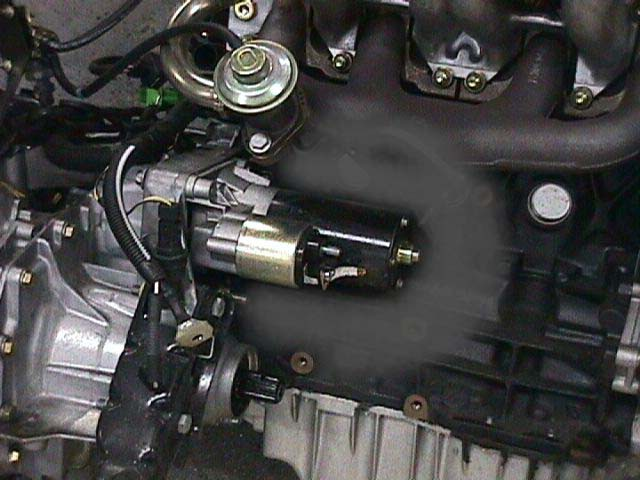
\includegraphics[width=0.6\linewidth]{img/demarreur.jpg}
  \caption{Démarreur}
  \label{img3}
\end{figure}

\subsection{Vérification de la tenue du palier 2}

Le démarreur D6RA n'a pas cessé d'évoluer depuis sa première version. La dernière évolution de ce modèle est le D6RA-100. Ce modèle, le plus puissant de la série, est destiné aux moteurs diesel de moyenne cylindrée. Le couple maximum sur l'arbre secondaire est alors de $C_{max} = 120 N.m$. Ce couple, plus important que sur le précédent modèle, engendre une augmentation de la pression de contact exercée par l'arbre 4 sur les paliers 2 et 24.

Afin de vérifier la tenue du palier 2, on demande de déterminer les torseurs d'actions mécaniques appliqués au système matériel $\left\{12+4\right\}$.

\newpage

Le schéma de modélisation statique est donné dans le document DR2/4. Les torseurs représentant les actions mécaniques appliquées au système matériel {12+4} sont les suivants :

\begin{figure}[!h]
  \begin{minipage}{0.48\linewidth}
  \begin{math}
  \left\{T_{64 \rightarrow \left\{12+4\right\}}\right\}=\left\{
  \begin{array}{c c}
  0 & -120 \\
  0 & 0 \\
  0 & 0
  \end{array}\right\}_{I,(\overrightarrow{x},\overrightarrow{y},\overrightarrow{z})}
  \end{math}
  \end{minipage}
  \hfill
  \begin{minipage}{0.48\linewidth}
  \begin{math}
  \left\{T_{1 \rightarrow \left\{12+4\right\}}\right\}=\left\{
  \begin{array}{c c}
  X_I & 0 \\
  Y_I & 0 \\
  Z_I & 0
  \end{array}\right\}_{I,(\overrightarrow{x},\overrightarrow{y},\overrightarrow{z})}
  \end{math}
\end{minipage}
\end{figure}

\begin{figure}[!h]
\begin{math}
  \left\{T_{1 \rightarrow \left\{12+4\right\}}\right\}=\left\{
  \begin{array}{c c}
  0 & 0 \\
  Y_G & 0 \\
  Z_G & 0
  \end{array}\right\}_{G,(\overrightarrow{x},\overrightarrow{y},\overrightarrow{z})}
\end{math}
\end{figure}

$\left\{T_{moteur \rightarrow \left\{12+4\right\}}\right\}_{(H,(\overrightarrow{x},\overrightarrow{y},\overrightarrow{z}))}$ torseur modélisant les actions mécaniques exercées par la couronne dentée du moteur sur le lanceur.

\paragraph{Question 1:} L'angle de pression de l'engrenage couronne moteur/$\left\{12+4\right\}$ est $\alpha=20$\textdegree.
Représenter, par un torseur, les actions mécaniques de la couronne du moteur sur $\left\{12+4\right\}$.
Écrire les composantes de ce torseur dans $(H,(\overrightarrow{x},\overrightarrow{y},\overrightarrow{z}))$.

\paragraph{Question 2:} Énoncer le Principe Fondamental de la Statique sur le système matériel $\left\{12+4\right\}$. Peut-on déterminer les actions mécaniques inconnues. Justifier la réponse.

Un logiciel de calcul informatique a permis de déterminer $Z_G = 7880 N$ et $Y_G = 2720 N$.

A l'aide des composantes de $\left\{T_{1 \rightarrow \left\{12+4\right\}}\right\}_{(G,(\overrightarrow{x},\overrightarrow{y},\overrightarrow{z}))}$, calculer la norme de l'effort radial dans le palier 2.

\paragraph{Question 3:} Les paliers sont dimensionné pour supporter un effort maxi de 8KN. Justifier du choix de ces paliers.

\newpage

\includepdf[landscape,pages=8]{img/Demarreur.pdf}
\includepdf[pages=9]{img/Demarreur.pdf}
%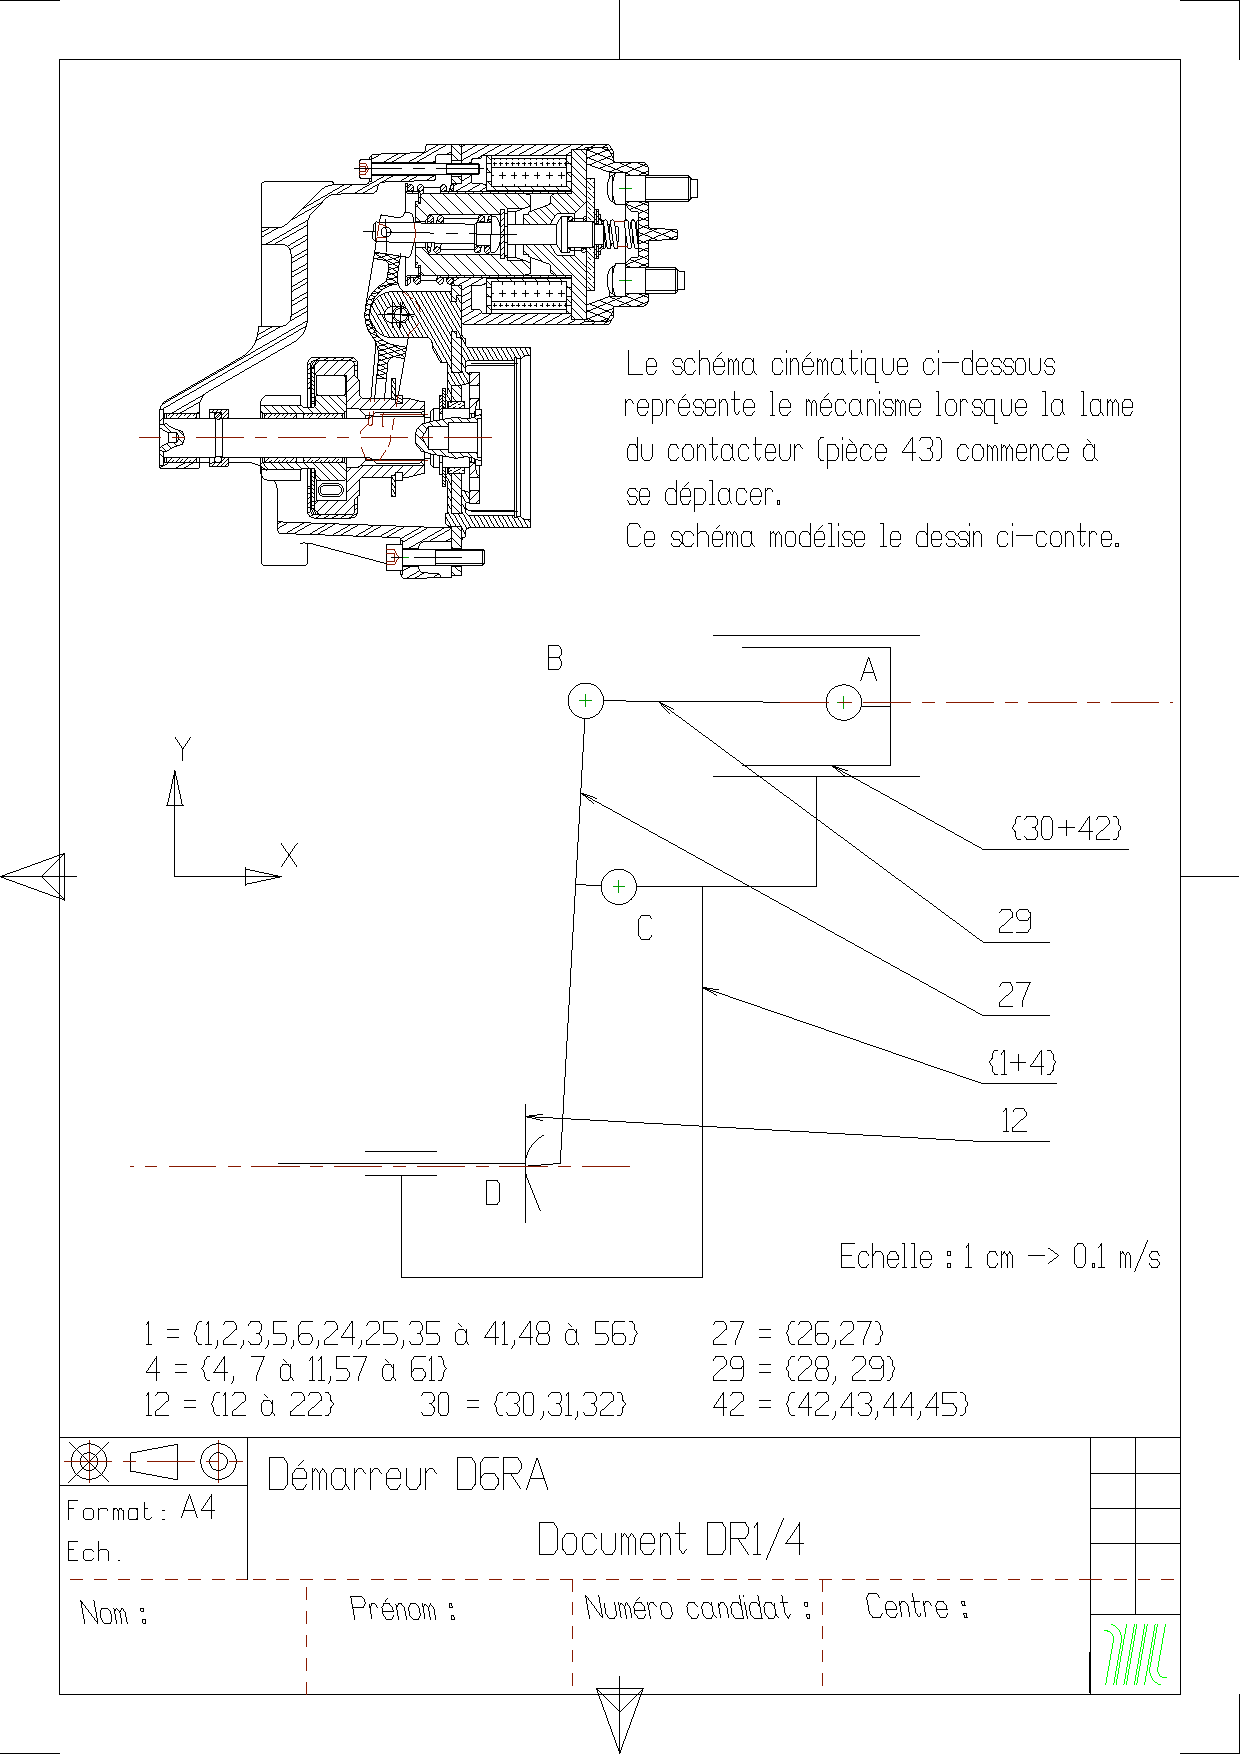
\includepdf{img/Dr1.pdf}
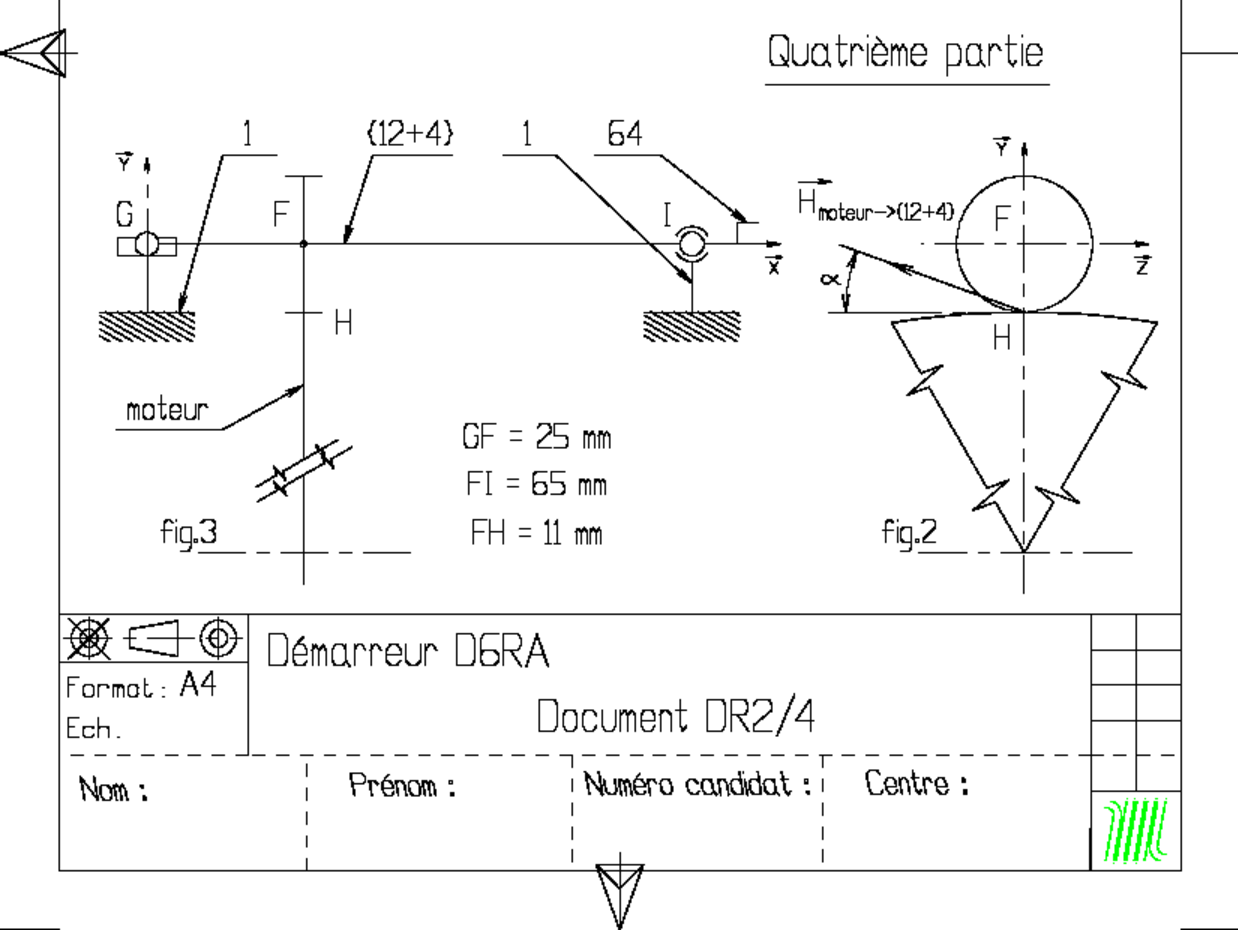
\includepdf{img/Dr2.pdf}

\newpage

\section{Siège de dentiste}

Le système étudié sera celui d'une chaise de dentiste dont la hauteur de la chaise est réglable afin de permettre une meilleure accessibilité. Le schéma cinématique du système de levée est donné à la figure \ref{chaise_cin}.

\begin{figure}[!h]
 \begin{minipage}{0.45\linewidth}
 \centering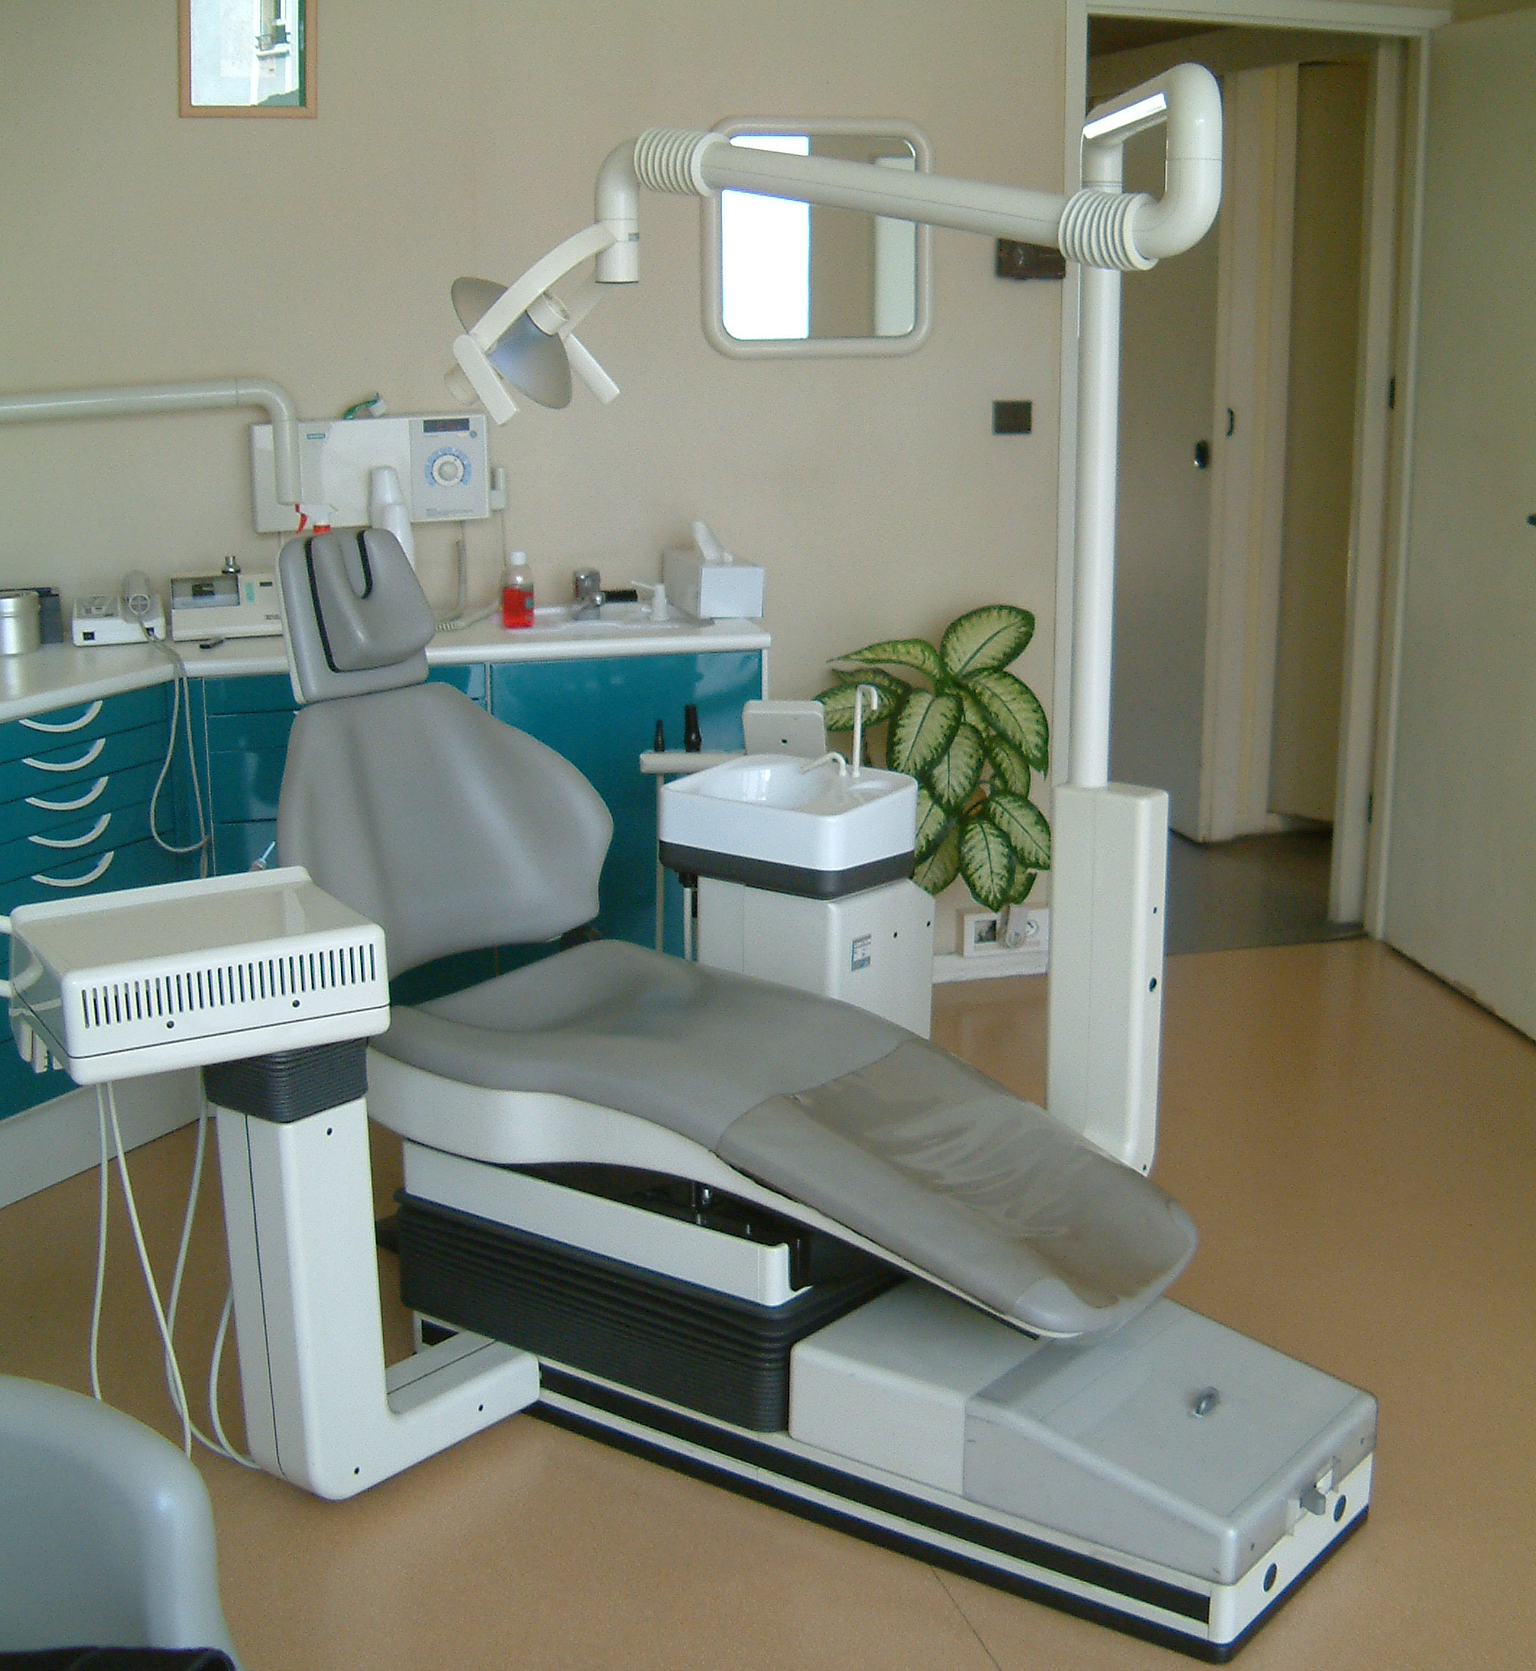
\includegraphics[height=50mm]{img/siege.png}
 \end{minipage}
 \hfill
 \begin{minipage}{0.45\linewidth}
 \centering\includegraphics[height=50mm]{img/siege_zoom.png}
 \end{minipage}
 \caption{Chaise de dentiste}
\end{figure}

\begin{figure}[!h]
 \begin{minipage}{0.55\linewidth}
 \centering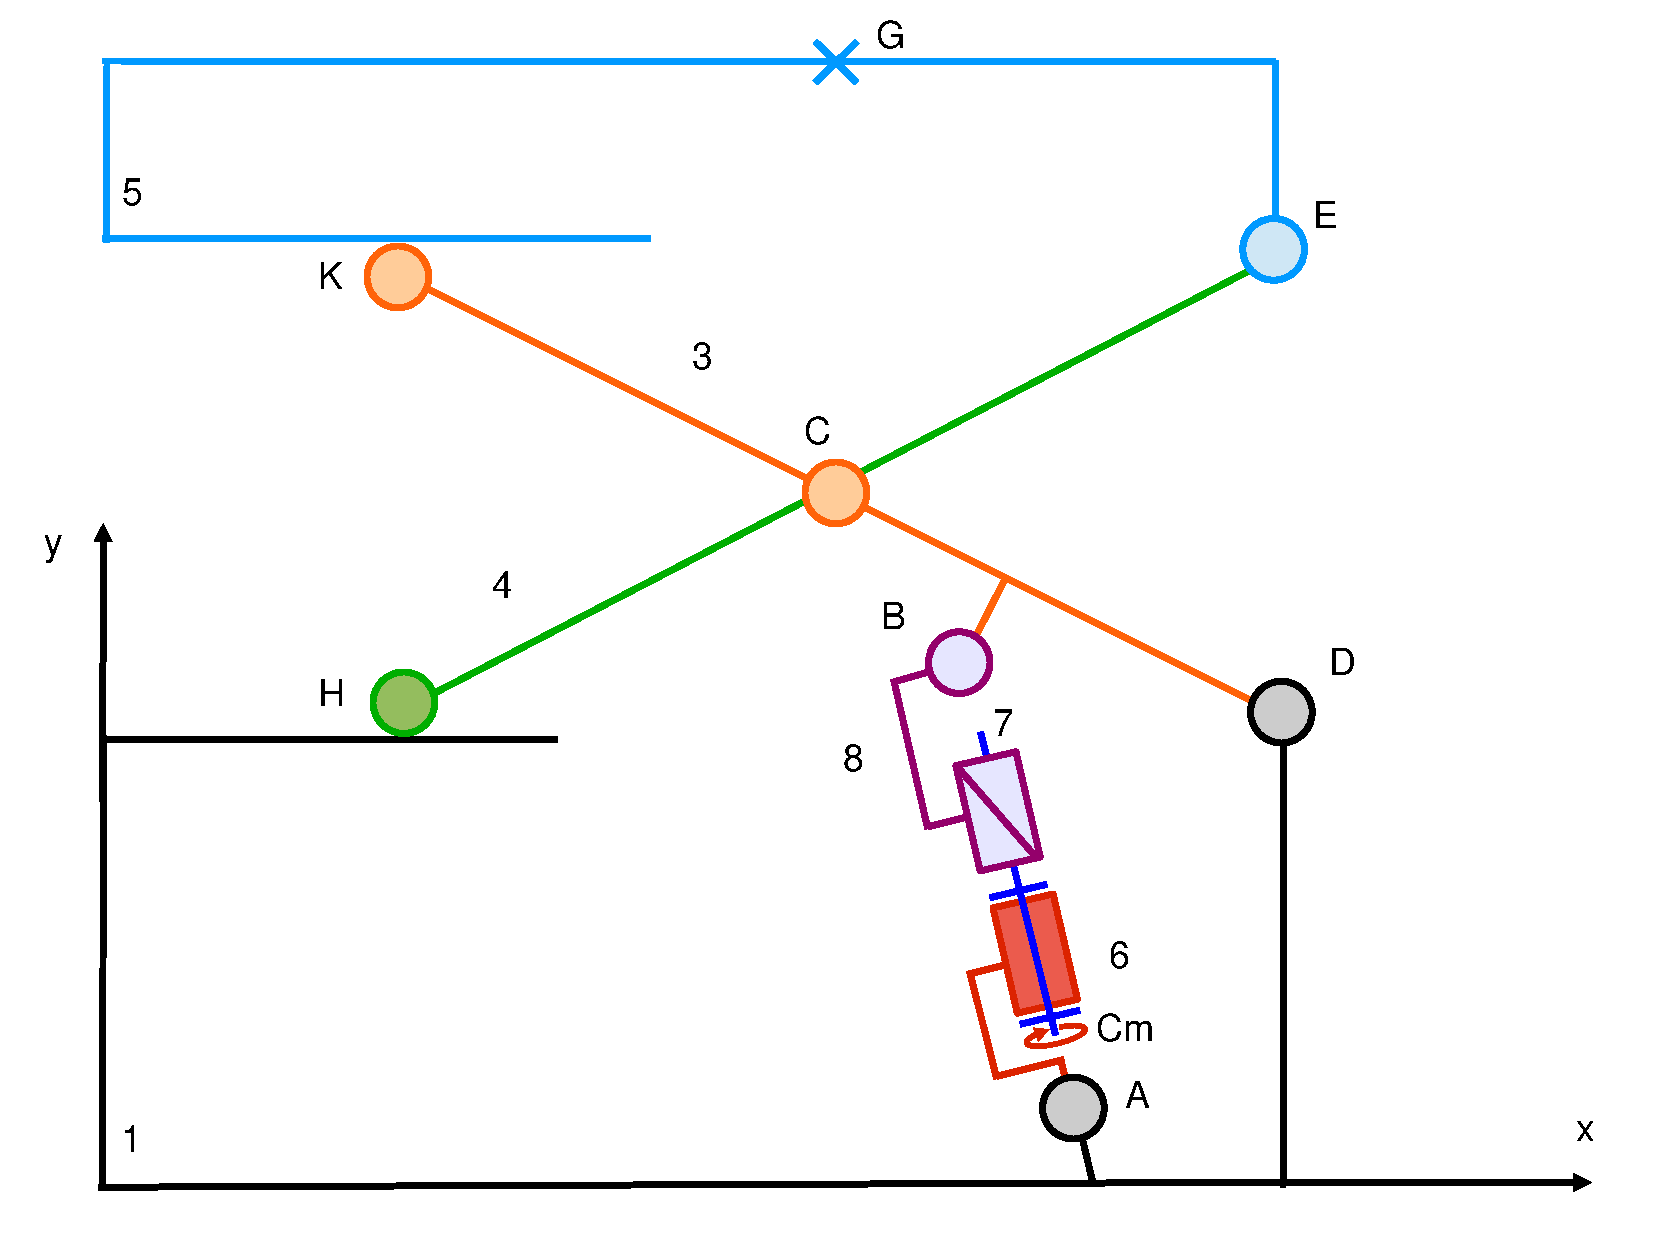
\includegraphics[width=\linewidth]{img/chaise_cin.pdf}
 \end{minipage}
 \hfill
 \begin{minipage}{0.48\linewidth}
\small Hypothèses simplificatrices et données : 
 \begin{itemize}
  \item Le point G matérialise la position de la charge que représente l'ensemble $\text{fauteuil + patient}$,
  \item Cette charge sera : $\overrightarrow{P_5}$, avec $\|\overrightarrow{P_5}\|=3000N$,
  \item Le poids des pièces est négligé devant les autres actions en présence,
  \item Le plan $(\overrightarrow{x},\overrightarrow{y})$ est plan de symétrie pour l'étude,
  \item Les liaisons entre les solides sont parfaites.
 \end{itemize}
 \end{minipage}
 \label{chaise_cin}
 \caption{Hypothèses et données}
\end{figure}

\normalsize

Les dimensions sont les suivantes:

\begin{itemize}
 \item $\overrightarrow{HC}=\overrightarrow{CE}=260.\overrightarrow{x}+100.\overrightarrow{y}$,
 \item $\overrightarrow{KC}=\overrightarrow{CD}=260.\overrightarrow{x}-100.\overrightarrow{y}$,
 \item $\overrightarrow{GE}=260.\overrightarrow{x}-50.\overrightarrow{y}$,
 \item $\overrightarrow{AB}=l.\overrightarrow{x_6}$,
 \item $\overrightarrow{CB}=50.\overrightarrow{x}-50.\overrightarrow{y}$,
 \item $(\overrightarrow{x},\overrightarrow{x_6})=\alpha=100\degree$,
 \item $p=4mm$
 \item Toute autre donnée qui sera jugée nécessaire pourra être ajoutée.
\end{itemize}

\paragraph{Question 1:} Représenter le graphe des liaisons de ce système.

\paragraph{Question 2:} Exprimer les torseurs des actions mécaniques de chacune des liaisons ainsi que ceux correspondants au poids du patient et au couple moteur.

\paragraph{Question 3:} Proposer un modèle permettant de déterminer l'action de la chaine de solides \{6,7,8\} sur 3.
 
\paragraph{Question 4:} Isoler la pièce 5, et déterminer les équations liées à l'isolement de cette pièce.

\paragraph{Question 5:} Isoler la pièce 4, et déterminer les équations liées à l'isolement de cette pièce.

\paragraph{Question 6:} Isoler la pièce 3, et déterminer les équations liées à l'isolement de cette pièce.

\paragraph{Question 7:} En déduire le couple du moteur qui permet de supporter le poids du patient.

Un logiciel de simulation informatique nous a permis d'obtenir les 2 courbes de la figure \ref{releves}.

\begin{figure}[!h]
 \begin{minipage}{0.45\linewidth}
 \centering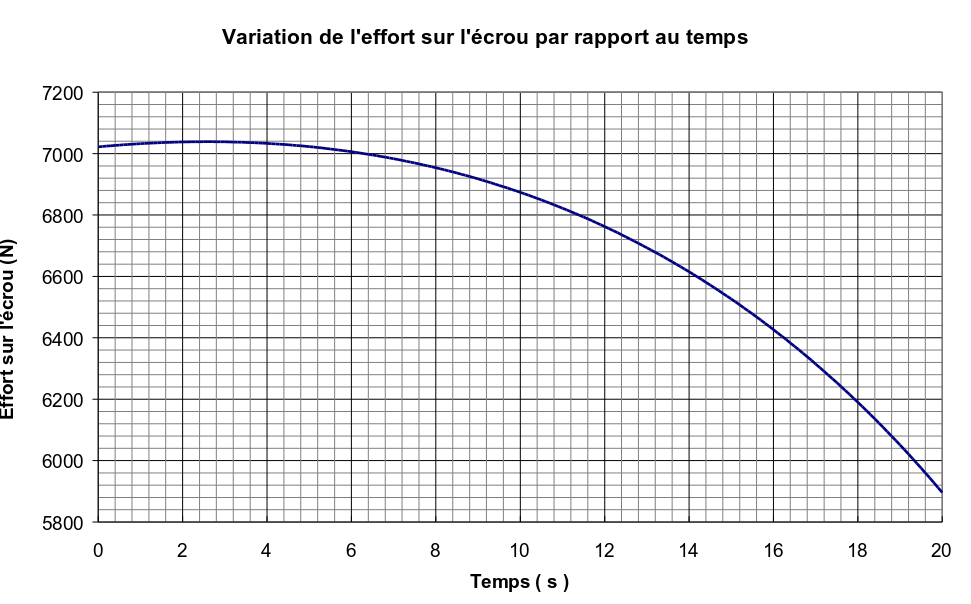
\includegraphics[width=0.9\linewidth]{img/courbe1.png}
 \end{minipage}
 \hfill
 \begin{minipage}{0.45\linewidth}
 \centering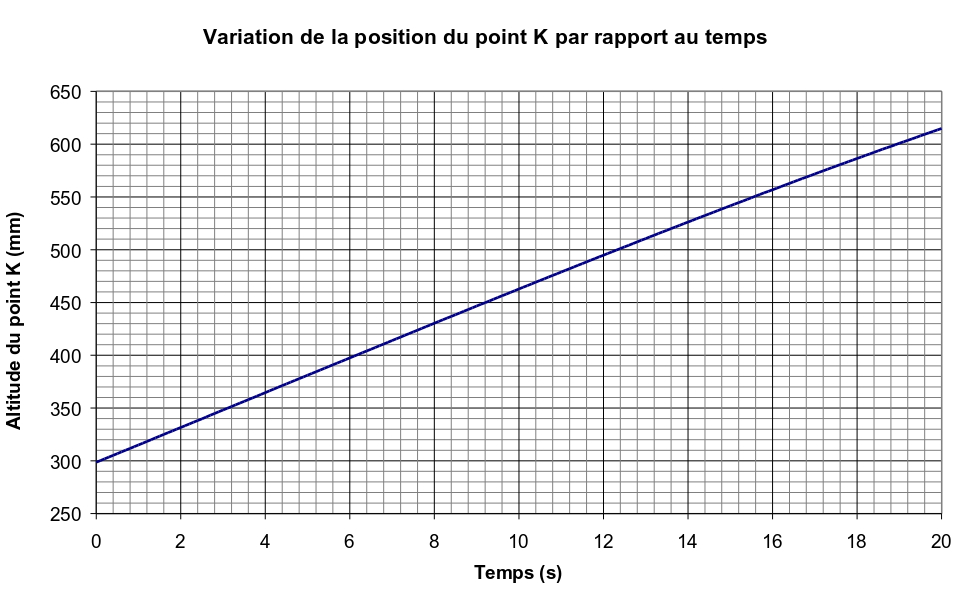
\includegraphics[width=0.9\linewidth]{img/courbe2.png}
 \end{minipage}
 \caption{Relevés du logiciel}
 \label{releves}
\end{figure}

\paragraph{Question 8:} Déterminez la valeur maximale de l'effort transmis par la charge à l'écrou : $\|\overrightarrow{B_{3\rightarrow E}}\|$.

\paragraph{Question 9:} Déduisez-en l'altitude du point K correspondant à l'effort maximum.

\newpage

\section{Robot Robuglass}

\subsection{Étude du fonctionnement global du système}

\begin{figure}[!h]
 \begin{minipage}{0.45\linewidth}
La société ROBOSOFT a développé le robot Robuglass, figure \ref{robuglass}, devant assurer de manière automatique l'entretien de la pyramide du Louvre sans nécessiter l'intervention (difficile et périlleuse) des opérateurs directement sur l'édifice.
 \end{minipage}
 \hfill
 \begin{minipage}{0.45\linewidth}
 \centering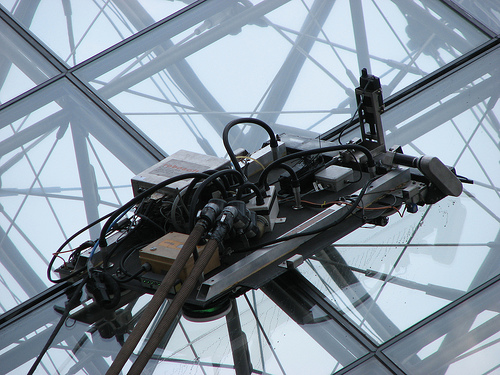
\includegraphics[width=0.9\linewidth]{img/robuglass.jpg}
 \end{minipage}
 \caption{Robot Robuglass}
 \label{robuglass}
\end{figure}


Le robot ROBUGLASS se compose de 4 sous ensembles distincts: 
\begin{itemize}
 \item le porteur: qui constitue le robot qui se déplace sur la surface vitrée,
 \item le chariot ombilical : qui supporte les 2 pompes à vide,
 \item le poste de contrôle : qui permet à l'opérateur de commander le porteur,
 \item le véhicule atelier : qui permet le rangement du porteur, de l'outillage et du chariot 
ombilical.
\end{itemize}

\subsection{Objectif: Vérification du critère de contact}
 
Pour un nettoyage efficace il est nécessaire de réguler l'effort d'application de la brosse sur la vitre. Un actionneur de type vérin électrique permet de mettre l'outil contenant la brosse en position haute ou basse et d'appliquer la brosse sur la surface vitrée avec l'effort requis.

L'effort maximum développé par le vérin est de 130 N. 



\begin{figure}[!h]
 \begin{minipage}{0.4\linewidth}
 \centering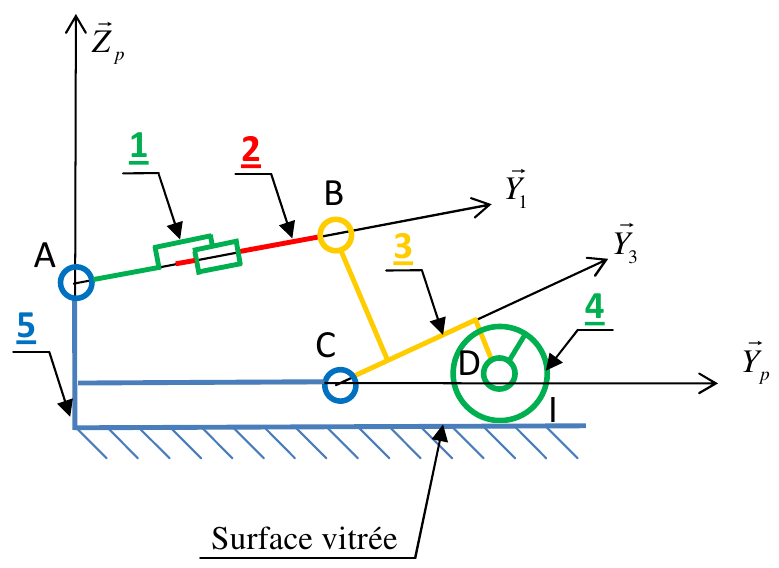
\includegraphics[width=\linewidth]{img/robuglass_cin.png}
 \end{minipage}
 \hfill
 \begin{minipage}{0.3\linewidth}
  \small
  \begin{itemize}
   \item $\overrightarrow{AB}=\lambda.\overrightarrow{Y_1}$,
   \item $\overrightarrow{AC}=a.\overrightarrow{Y_p}-b.\overrightarrow{Z_p}$,
   \item $\overrightarrow{CB}=c.\overrightarrow{Y_3}+d.\overrightarrow{Z_3}$,
   \item $\overrightarrow{CD}=e.\overrightarrow{Y_3}-f.\overrightarrow{Z_3}$,
   \item $\overrightarrow{ID}=r_4.\overrightarrow{Z_p}$,
   \item $\theta_1=\left(\overrightarrow{Y_p},\overrightarrow{Y_1}\right)=15\degree$,
   \item $\theta_3=\left(\overrightarrow{Y_p},\overrightarrow{Y_3}\right)=30\degree$,
   \end{itemize}
 \end{minipage}
  \hfill
 \begin{minipage}{0.25\linewidth}
  \begin{itemize}
   \item $a=360mm$,
   \item $b=120mm$,
   \item $c=40mm$,
   \item $d=130mm$,
   \item $e=120mm$,
   \item $f=50mm$,
   \item $r_4=30mm$.
   \end{itemize}
 \end{minipage}
 \caption{Schéma cinématique du Robot Robuglass}
 \label{robuglass_cin}
\end{figure}

On rappelle: $cos15\degree=0.96$, $sin15\degree=0.26$, $cos30\degree=\frac{\sqrt{3}}{2}$, $sin30\degree=\frac{1}{2}$.
 
Le vérin (voir Annexe 3, figure 4) est modélisé par le corps 1 et la tige 2 respectivement en liaison pivot d'axe $(A,\overrightarrow{X_p})$ et $(B,\overrightarrow{X_p})$ avec le porteur 5 (considéré comme fixe par rapport à la surface vitrée 0), et le support d'outil 3. Ce dernier est en liaison pivot d'axe $(C,\overrightarrow{X_p})$ avec le porteur. La brosse 4 est en liaison pivot d'axe $(D,\overrightarrow{X_p})$ avec le support d'outil 3. Le point de contact entre la brosse 4 et la surface vitrée fixe 0 est noté I (Document Réponse B9). 

L'objectif est de déterminer l'effort développé par le vérin. On négligera les effets du poids sur l'ensemble des pièces de l'outil. On notera les actions mécaniques d'un solide $i$ sur un solide $j$ : $\overrightarrow{F_{i\rightarrow j}}$. L'action  $\overrightarrow{F_{5\rightarrow 4}}$ appliquée au point I est donnée par: $\overrightarrow{F_{5\rightarrow 4}}=-20.\overrightarrow{Y_p}+100.\overrightarrow{Z_p}$. Le problème peut être résolu sous les hypothèses de statique plane. 
 
\paragraph{Question 1:} Isoler l'ensemble $\left\{1,2\right\}$, établir les 3 équations qui lient les composantes des torseurs statiques.

\paragraph{Question 2:} Isoler l'ensemble $\left\{3,4\right\}$, établir les 3 équations qui lient les composantes des torseurs statiques.
 
\paragraph{Question 3:} En déduire l'action $\overrightarrow{F_{3\rightarrow 2}}$ et donc l'effort dans le vérin. Cette valeur est-elle compatible avec le vérin utilisé.

\ifdef{\public}{\end{document}}{}

\clearpage

\newpage

\section{Correction}

\subsection{Colleuse de lamelle}

\paragraph{Question 2:} 

$\left\{T_{0\rightarrow 10}\right\}=\left\{
\begin{array}{cc}
X_{010} & L_{010} \\
Y_{010} & 0 \\
Z_{010} & N_{010}
\end{array}
\right\}_{O,R_0}$

$\left\{T_{10\rightarrow 11}\right\}=\left\{
\begin{array}{cc}
X_{1011} & L_{1011} \\
Y_{1011} & M_{1011} \\
Z_{1011} & N_{1011}
\end{array}
\right\}_{O,R_0}$, avec $M_{1011}=\frac{P}{2.\pi}.Y_{1011}$

$\left\{T'_{0\rightarrow 11}\right\}=\left\{
\begin{array}{cc}
X'_{011} & L'_{011} \\
0 & 0 \\
Z'_{011} & N'_{011}
\end{array}
\right\}_{B,R_0}=\left\{
\begin{array}{cc}
X'_{011} & L'_{011}+\mu.Z'_{011} \\
0 & a.Z'_{011} \\
Z'_{011} & N'_{011}-\mu.X'_{011}
\end{array}
\right\}_{B,R_0}$

$\left\{T''_{0\rightarrow 11}\right\}=\left\{
\begin{array}{cc}
X''_{011} & L''_{011}+\mu.Z''_{011} \\
0 & -a.Z''_{011} \\
Z''_{011} & N''_{011}-\mu.X''_{011}
\end{array}
\right\}_{C,R_0}$


\paragraph{Question 3:}

Isoler 10.

$\left\{\begin{array}{l}
X_{010}-X_{1011}=0 \\
Y_{010}-Y_{1011}=0 \\
Z_{010}-Z_{1011}=0 \\
L_{010}-L_{1011}=0 \\
0-M_{010}+C_m=0  \\
N_{010}-N_{1011}=0 \\
\end{array}\right.$

\paragraph{Question 4:}

Isoler 11.

$\left\{\begin{array}{l}
X'_{011}+X''_{011}+X_{1011}=0 \\
Y_{1011}-P=0 \\
Z'_{011}+Z''_{011}+Z_{1011}=0 \\
L'_{011}+\mu.Z'_{011}+L''_{011}+\mu.Z''_{011}+L_{1011}=0 \\
a.Z'_{011}-a.Z''_{011}0+M_{010}=0  \\
-\mu.X'_{011}-\mu.X''_{011}+N_{010}=0
\end{array}\right.$

\paragraph{Question 5:}

$Cm=\frac{p}{2.\pi}.P=0,1N.m$

Le couple nominal est donc suffisant.

\subsection{Démarreur D6RA}

\paragraph{Question 1:}

$\left\{T_{mot\rightarrow 12+4}\right\}=\left\{
\begin{array}{cc}
0 & 0 \\
sin\alpha.\|\overrightarrow{H_{mot\rightarrow 12+4}}\| & 0 \\
-cos\alpha.\|\overrightarrow{H_{mot\rightarrow 12+4}}\| & 0
\end{array}
\right\}_{H,R}$

\paragraph{Question 2:}

$\left\{T_{mot\rightarrow 12+4}\right\}=\left\{
\begin{array}{cc}
0 & FH.cos\alpha.\|\overrightarrow{H_{mot\rightarrow 12+4}}\| \\
sin\alpha.\|\overrightarrow{H_{mot\rightarrow 12+4}}\| & 0 \\
-cos\alpha.\|\overrightarrow{H_{mot\rightarrow 12+4}}\| & 0
\end{array}
\right\}_{F,R}$

$\left\{T_{1\rightarrow 12+4}\right\}=\left\{
\begin{array}{cc}
X_I & 0 \\
Y_I & -FI.Z_I \\
Z_I & FI.Y_I
\end{array}
\right\}_{F,R}$

$\left\{T_{1\rightarrow 12+4}\right\}=\left\{
\begin{array}{cc}
0 & 0 \\
Y_G & FG.Z_G \\
Z_G & -FG.Y_G
\end{array}
\right\}_{F,R}$

$\left\{T_{mot\rightarrow 12+4}\right\}=\left\{
\begin{array}{cc}
0 & -120 \\
0 & 0 \\
0 & 0
\end{array}
\right\}_{F,R}$


$\left\{
X_I=0 \\
sin\alpha.\|\overrightarrow{H_{mot\rightarrow 12+4}}\|+Y_I+Y_G=0 \\
-cos\alpha.\|\overrightarrow{H_{mot\rightarrow 12+4}}\|+Z_I+Z_G=0 \\
FH.cos\alpha.\|\overrightarrow{H_{mot\rightarrow 12+4}}\|-120=0 \\
-FI.Z_I+FG.Z_G=0 \\
FI.Y_I-FG.Y_G=0
\right.$

Donc, $H=\frac{120}{FH.cos\alpha}$

$\left\{\begin{array}{l}
Y_I=-Y_G-sin\alpha.\frac{120}{FH.cos\alpha}\approx -6720N \\
Z_I=-Z_G+\frac{120}{FH}\approx 3120N
\end{array}\right.$

La norme est donc $\sqrt{Y_I^2+Z_I^2}=\sqrt{6720^2+3120^2}\approx 7400N$, les paliers sont donc bien dimensionnés.

\subsection{Siège de dentiste}

\paragraph{Question 2:}

$\left\{T_{1\rightarrow 3}\right\}=\left\{
\begin{array}{cc}
X_{13} & \sim \\
Y_{13} & \sim \\
\sim & 0
\end{array}
\right\}_{D,R}$

$\left\{T_{1\rightarrow 4}\right\}=\left\{
\begin{array}{cc}
0 & \sim \\
Y_{14} & \sim \\
\sim & 0
\end{array}
\right\}_{H,R}$

$\left\{T_{3\rightarrow 5}\right\}=\left\{
\begin{array}{cc}
0 & \sim \\
Y_{35} & \sim \\
\sim & 0
\end{array}
\right\}_{K,R}$

$\left\{T_{4\rightarrow 5}\right\}=\left\{
\begin{array}{cc}
X_{45} & \sim \\
Y_{45} & \sim \\
\sim & 0
\end{array}
\right\}_{E,R}$

$\left\{T_{P\rightarrow 5}\right\}=\left\{
\begin{array}{cc}
0 & \sim \\
-P & \sim \\
\sim & 0
\end{array}
\right\}_{G,R}$

$\left\{T_{3\rightarrow 4}\right\}=\left\{
\begin{array}{cc}
X_{34} & \sim \\
Y_{34} & \sim \\
\sim & 0
\end{array}
\right\}_{C,R}$

\paragraph{Question 3:}

La chaine de solides peut être considérée comme un vérin électrique. La norme de l'effort est $\frac{C_m.2.\pi}{p}$ et sa direction est $\overrightarrow{x_6}$.

$\left\{T_{verin \rightarrow 3}\right\}=\left\{
\begin{array}{cc}
\frac{C_m.2.\pi}{p} & \sim \\
0 & \sim \\
\sim & 0
\end{array}
\right\}_{B,R_6}$


\paragraph{Question 4:}

Isoler 5

$\left\{T_{3\rightarrow 5}\right\}=\left\{
\begin{array}{cc}
0 & \sim \\
Y_{35} & \sim \\
\sim & -260.Y_{35}
\end{array}
\right\}_{G,R}$

$\left\{T_{4\rightarrow 5}\right\}=\left\{
\begin{array}{cc}
X_{45} & \sim \\
Y_{45} & \sim \\
\sim & 260.Y_{45}+50.X_{45}
\end{array}
\right\}_{G,R}$

$\left\{\begin{array}{l}
X_{45}=0 \\
Y_{35}+Y_{45}-P=0 \\
260.Y_{45}+50.X_{45}-260.Y_{35}=0
\end{array}\right.$

Donc, $\left\{\begin{array}{l}
X_{45}=0 \\
Y_{35}=Y_{45}=\frac{P}{2}
\end{array}\right.$

\paragraph{Question 5:}

Isoler 4

En prenant en compte les résultats précédents.

$\left\{T_{4\rightarrow 5}\right\}=\left\{
\begin{array}{cc}
0 & \sim \\
\frac{P}{2} & \sim \\
\sim & 130.P
\end{array}
\right\}_{C,R}$

$\left\{T_{1\rightarrow 4}\right\}=\left\{
\begin{array}{cc}
0 & \sim \\
Y_{14} & \sim \\
\sim & -260.Y_{14}
\end{array}
\right\}_{C,R}$

$\left\{\begin{array}{l}
X_{34}=0 \\
Y_{34}-\frac{P}{2}+Y_{14}=0 \\
-130.P-260.Y_{14}=0
\end{array}\right.$

Donc, $\left\{\begin{array}{l}
X_{34}=0 \\
Y_{14}=-\frac{P}{2} \\
Y_{34}=P
\end{array}\right.$

\paragraph{Question 6:}

Isoler 3

En prenant en compte les résultats précédents.

$\left\{T_{5\rightarrow 3}\right\}=\left\{
\begin{array}{cc}
0 & \sim \\
-\frac{P}{2} & \sim \\
\sim & 130.P
\end{array}
\right\}_{C,R}$

$\left\{T_{1\rightarrow 3}\right\}=\left\{
\begin{array}{cc}
X_{13} & \sim \\
Y_{13} & \sim \\
\sim & 260.Y_{13}+100.X_{13}
\end{array}
\right\}_{C,R}$

$\left\{T_{verin \rightarrow 3}\right\}=\left\{
\begin{array}{cc}
\frac{Cm.2.\pi}{p} & \sim \\
0 & \sim \\
\sim & 0
\end{array}
\right\}_{B,R_6}=\left\{
\begin{array}{cc}
\frac{Cm.2.\pi}{p}.cos\alpha & \sim \\
\frac{Cm.2.\pi}{p}.sin\alpha & \sim \\
\sim & 0
\end{array}
\right\}_{B,R}$

$\left\{T_{verin \rightarrow 3}\right\}=\left\{
\begin{array}{cc}
\frac{Cm.2.\pi}{p}.cos\alpha & \sim \\
\frac{Cm.2.\pi}{p}.sin\alpha & \sim \\
\sim & (50.cos\alpha+50.sin\alpha).\frac{Cm.2.\pi}{p}
\end{array}
\right\}_{C,R}$

$\left\{T_{4\rightarrow 3}\right\}=\left\{
\begin{array}{cc}
0 & \sim \\
-P & \sim \\
\sim & 0
\end{array}
\right\}_{C,R}$

$\left\{\begin{array}{l}
X_{13}+\frac{C_m.2.\pi.cos\alpha}{p}=0 \\
Y_{13}-\frac{P}{2}+\frac{C_m.2.\pi.qin\alpha}{p}-P=0 \\
130.P+260.Y_{13}+100.X_{13}+(50.cos\alpha+50.sin\alpha).\frac{C_m.2.\pi}{p}=0
\end{array}\right.$

$520.P=(210.sin\alpha+50.cos\alpha).\frac{C_m.2.\pi}{p}$

$C_m=\frac{p}{2.\pi}.\frac{520}{210.sin\alpha+50.cos\alpha}.P$

$C_m\approx 5N.m$

\subsection{Robot Robuglass}

\paragraph{Question 1:}

Isoler 1 et 2

$\left\{T_{5\rightarrow 1}\right\}=\left\{
\begin{array}{cc}
\sim & 0 \\
Y_{51} & \sim \\
Z_{51} & \sim
\end{array}
\right\}_{A,R_1}$

$\left\{T_{3\rightarrow 2}\right\}=\left\{
\begin{array}{cc}
\sim & 0 \\
Y_{32} & \sim \\
Z_{32} & \sim
\end{array}
\right\}_{B,R_1}=\left\{
\begin{array}{cc}
\sim & \lambda.Z_{32} \\
Y_{32} & \sim \\
Z_{32} & \sim
\end{array}
\right\}_{A,R_1}$

Donc,

$\left\{\begin{array}{l}
Y_{51}+Y_{32}=0 \\
Z_{51}+Z_{32}=0
\end{array}\right.$, ainsi $\left\{\begin{array}{l}
Y_{51}=-Y_{32}=F_{verin} \\
Z_{51}=Z_{32}=0
\end{array}\right.$

\paragraph{Question 2:}

Isoler 3 et 4

En prenant en compte les résultats précédents.

$\left\{T_{2\rightarrow 3}\right\}=\left\{
\begin{array}{cc}
\sim & 0 \\
F_{verin} & \sim \\
0 & \sim
\end{array}
\right\}_{B,R_1}=\left\{
\begin{array}{cc}
\sim & 0 \\
cos\theta_1.F_{verin}  & \sim \\
sin\theta_1.F_{verin}  & \sim
\end{array}
\right\}_{B,R_p}=\left\{
\begin{array}{cc}
\sim & X \\
cos\theta_1.F_{verin} & \sim \\
sin\theta_1.F_{verin} & \sim
\end{array}
\right\}_{B,R_p}$

avec $X=-\left[c.sin(\theta_3-\theta_1)+d.cos(\theta_3-\theta_1)\right].F_{verin}$

$\left\{T_{5\rightarrow 3}\right\}=\left\{
\begin{array}{cc}
\sim & 0 \\
Y_{53} & \sim \\
Z_{53} & \sim
\end{array}
\right\}_{C,R_p}$

$\left\{T_{5\rightarrow 4}\right\}=\left\{
\begin{array}{cc}
\sim & 0 \\
-20 & \sim \\
100 & \sim
\end{array}
\right\}_{I,R_p}=\left\{
\begin{array}{cc}
\sim & Y \\
-20 & \sim \\
100 & \sim
\end{array}
\right\}_{I,R_p}$

avec $Y=(100.e-20.f).cos\theta_3+(100.f+20.e).sin\theta_3-20.r_4$

Donc,

$\left\{\begin{array}{l}
Y_{53}-20+cos\theta_1.F_{verin}=0 \\
Z_{53}+100+sin\theta_1.F_{verin}=0 \\
X+Y=0
\end{array}\right.$

Donc, $F_{verin}=\frac{(100.e-20.f).cos\theta_3+(100.f+20.e).sin\theta_3-20.r_4}{c.sin(\theta_3-\theta_1)+d.cos(\theta_3-\theta_1)}$

$F_{verin}=\frac{(100.120-20.50).cos30\degree+(100.50+20.120).sin30\degree-20.30}{40.sin15\degree+130.cos15\degree}$

$F_{verin}=92,89N$

\end{document}
